% Gene co-expression networks: https://en.wikipedia.org/wiki/Gene_co-expression_network#:~:text=Having%20gene%20expression%20profiles%20of,rise%20and%20fall%20together%20across

The cost of producing data has plummeted in recent years and many people are capitalizing on technological advancements to do so. In the field of genomics, the sequencing of the first human genome (2002) took around years and cost over \$3 million to complete. Nowadays, it is possible to sequence hundreds of genomes in just a few days with a cost of around \$1,000 each \cite{big_biological_impacts_bd}. However, the vast amounts of data that are produced can result in a problem: data information overload. To solve this, new visualization tools are needed to help examine large volumes of data so that novel patterns in them can be found, which in turn will lead to new scientific discoveries.

% These problems can be overcome with a visualization system that can scale to large sizes of data and where the interactions are not cumbersome. In this way, we can visualize the data in order to find interesting patterns that will lead to new scientific discoveries
%  \cite{zhang_paciorkowski_craig_cui_2019}.

% Some of the main problems that researchers face when analysing genomic data are: information overload, data interconnectivity and high dimensionality. One way to deal with all this data is to invent novel analysis. However, we still need visual inspection of the data, which is an important challenge, and this is what we attempt to solve. For this reason, it is very important to implement efficient visualization technologies that can lead to find new patterns and the extraction of good conclusions of the data.

In the field of system biology, there are usually network representations where the nodes or bioentities are connected to each other. These connections represent associations. Networks can increase dramatically in size and complexity and many visualization systems for biological networks lack scalability and the user interactions can be cumbersome. Virtual Reality (VR) has shown to have benefits when visualizing abstract information and offers rich interactivity \cite{zhang_paciorkowski_craig_cui_2019}. Some specific challenges that we face when visualizing biological networks in VR are the following:
\begin{itemize}
  \item Information overload because of the large number of nodes, edges, and information connected to those such as the weights and modules when visualizing large biological networks in Virtual Reality.
  \item Understanding the scalability limitations as for the number of nodes and edges for the exploration of biological networks in VR.
  \item Performance requirements needed (72 FPS), so that the interactions are not cumbersome, using inexpensive VR equipment.
\end{itemize}

% enough computational power to create these large networks, scientific knowledge about large networks a. We need better visualization systems for the analysis and inspection of biological networks and at the same time we need robust applications that can handle the data overload.

There are existing approaches for the visualization of large biological networks, but the have limitations. Many of them are 2-dimensional, some provide a 3-dimensional view and a limited number of them are compatible with Virtual Reality. These tools struggle with information overload problems or the "hairball" effect when the network becomes larger. Some tools like Cytoscape \cite{cytoscape}, NAViGaTOR \cite{navigator} or BioLayoutExpress3D \cite{biolayout3d}, help overcome these problems with specific hardware or libraries, other tools just trade off the interactivity in favour of showing large amounts of data \cite{agapito_guzzi_cannataro_2013}.


%[What I expect to read here is why your solution is better than the previous solutions described in the previous section.]


We have implemented GeneNet VR, a virtual reality application for the visualization of large biological networks. We used two datasets from the MIxT project \cite{dumeaux_fjukstad_interactions_tumor_blood} that contain genetic information from patients with breast cancer. MIxT provides a 2-dimensional visualization tool to explore these datasets. However, it has some known visual and scalability problems. With GeneNet VR, we overcome these problems by providing the following solutions:
\begin{enumerate}
  \item Visualization of the network in a three-dimensional immersive space and implementation of interactive and visual solutions to reduce information overload.
  \item Design and implementation guidelines based on the evaluation results.
  \item Implementation for the Oculus Quest, a cheap Virtual Reality headset.
\end{enumerate}

We evaluated the performance of GeneNet VR and several of the interaction that are commonly used for network exploration. Another experiment was also carried out to evaluate the performance of the application on the Oculus Quest hardware. We concluded from the experiments that GeneNet VR performs well for the network sizes that we tested and that the interactions with the network achieved the required Frames Per Second (FPS) defined by Oculus. We also concluded that we can use inexpensive VR hardware to explore biological networks.

To evaluate the quality of GeneNet VR, we used a qualitative research where data was collected using semi-structured interviews with several scientific researchers. The feedback that we obtained was positive, hightlighting that the application is helpful for the visualization of biological networks and easy to learn even for novice VR users.

\textbf{Thesis statement: } \emph{Virtual Reality is advantageous for the visualization of large biological networks and for rapid exploration of patterns in them using affordable hardware}.

\section{Challenges and research problem}

In fields such as biology, network visualization seems to be particularly helpful \cite{pujana_network_modeling} \cite{fraser_view_function}. There are many types of relationships that can be measured in a biological context, for example interactions between proteins or genetic interections when revealed by combinations of mutations. All these interactions and correlations can be easier to visualize as a network \cite{merico_visualization}.

MIxT \cite{fjukstad_dumeaux_olsen_lund_hallett_bongo_2017} is a web application for bioinformaticians that is used to identify genes and pathways in a primary tumor that are tightly linked to genes and pathways in the systemic response of a patient with breast cancer \cite{dumeaux_fjukstad_interactions_tumor_blood}. Among other tools, it offers a visualization tool for the biological networks where the nodes are genes and the edges between two nodes represent a statistically significant correlation in expression between them.

OmicsNet is another example of a visualization tool with data overload problems \cite{omnicsnet}. OmicsNet is a web application for creating different types of molecular interaction networks and visually exploring them in a three-dimensional space. However, the application also struggles with problems like edge occlusion and performance, making it hard to visualize the network when they become larger.

It can be hard to identify novel patterns when exploring large amounts of data. Some data structures, like the networks, also have the challenge of data interconnectivity. These data structures represent relationships and are composed of nodes and edges. Even though we have many tools like machine learning that help researchers automate and accelerate the identification of patterns, we still need expert human involvement expert to check and inspect these networks \cite{network_expert}.

When exploring a network in MIxT, sometimes it can be difficult to find patterns because of the data overload issues. This problem happens particularly when there are many interconnecting nodes. In figure \ref{fig:mixt_network} we can see an example of the network visualization from MIxT. As we can see in Figure \ref{fig:mixt_network1}, there are many interconnecting nodes; this problem is amplified when we zoom into the network as in Figure \ref{fig:mixt_network_zoom}.

\begin{figure}[h!]
    \centering%
    \begin{subfigure}[t]{0.5\textwidth}
        \centering%
        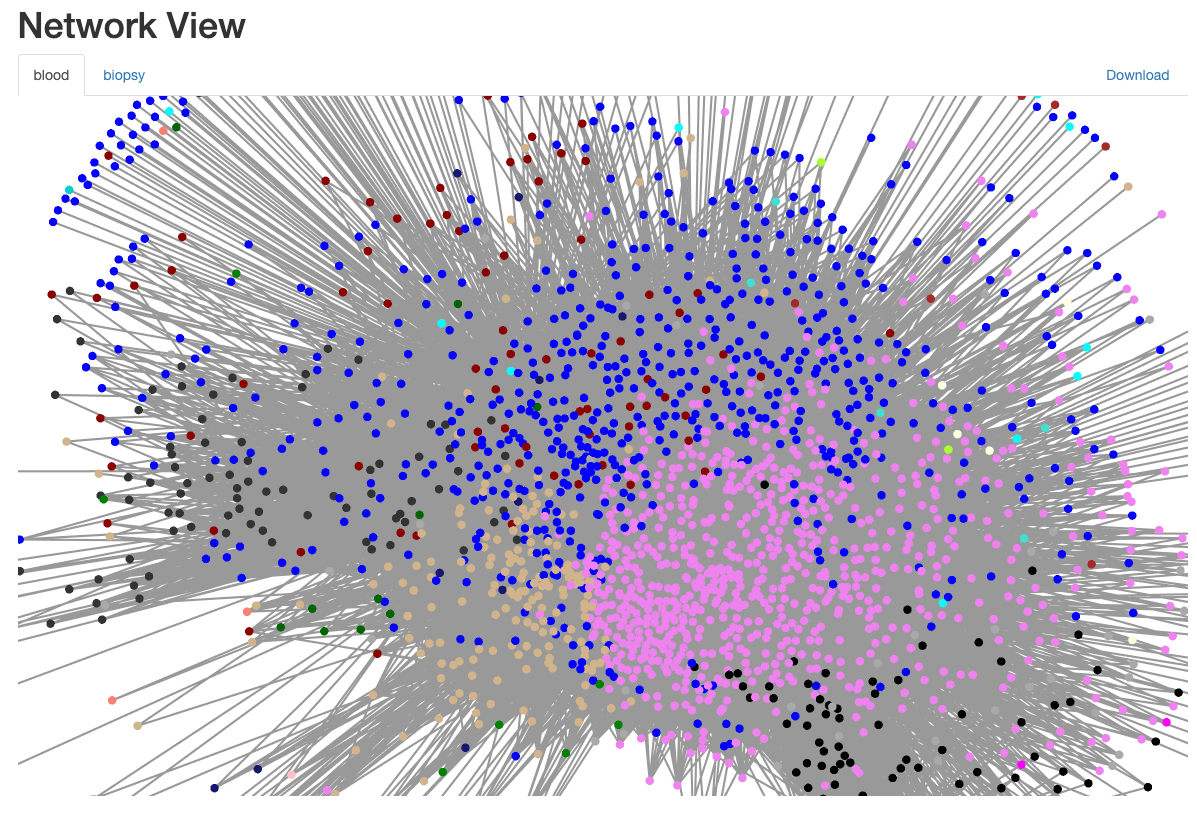
\includegraphics[width=\linewidth]{mixt_network1}
        \caption{Network with several modules.}
        \label{fig:mixt_network1}
    \end{subfigure}%
    \begin{subfigure}[t]{0.5\textwidth}
        \centering%
        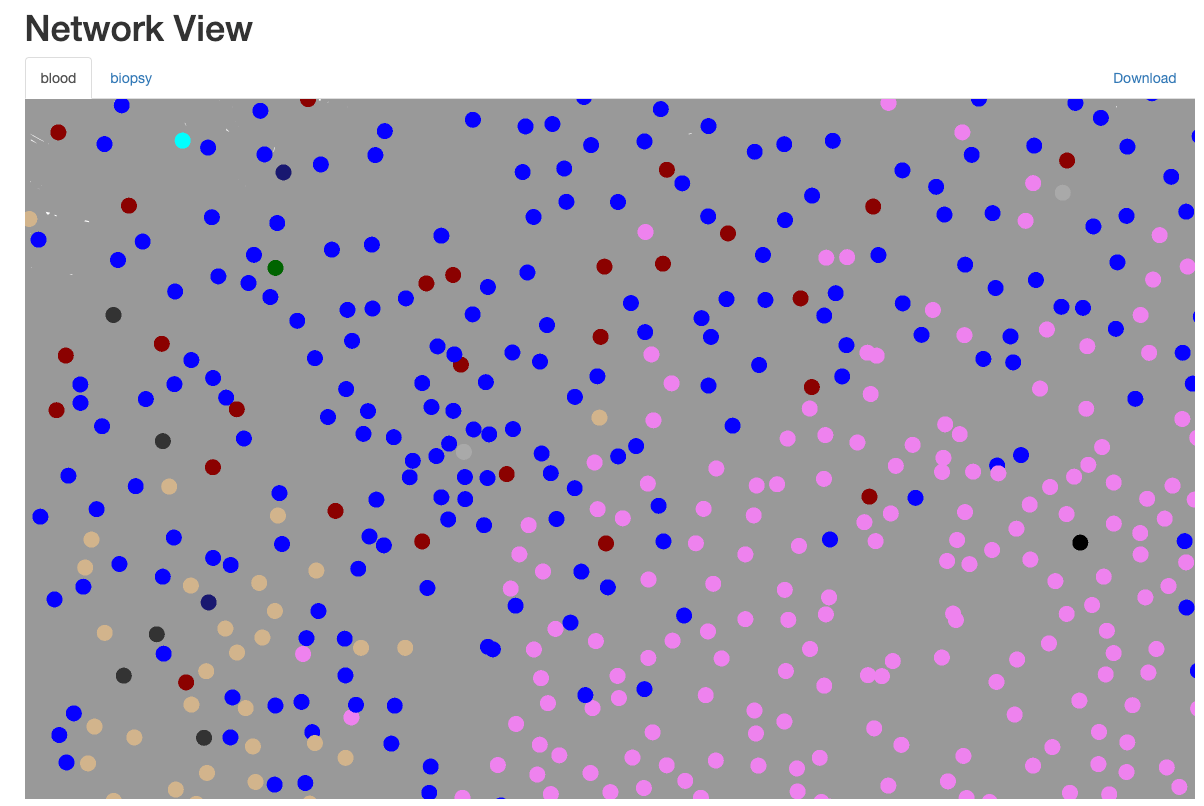
\includegraphics[width=\linewidth]{mixt_network2}
        \caption{More focused image of the network.}
        \label{fig:mixt_network_zoom}
    \end{subfigure}

    \caption{Network view of the MIxT application where nodes represent genes and the modules are represented by colors. Relationships are represented by grey lines that connect one gene to another.}
    \label{fig:mixt_network}
\end{figure}

There are additional challenges when exploring large biological networks in Virtual Reality. When we are in an immersive three-dimensional space, we have occlusion problems. This occurs, for example, when the nodes or edges that we have in front of us hide or obscure other nodes or edges that are behind them. One solution can be to show the network from another angle. We can do this by rotating and moving the network or by making it possible for the user to move to other parts in the virtual world. With reference to the issue of information overload, as highlighted earlier, this can be resolved by showing only the information that the user needs to visualize at any given time. This can be done by filtering the data so that we can focus on what we are interested in.

The interactivity in VR is usually done with the VR controllers, which simulate our hands in the virtual world. We can implement natural actions for the operator such as grabbing objects or items with their hands, which will feel intuitive. However, we can also implement other actions in the virtual world like using laser pointers to select something, using 2D menus inside the virtual world or teleporting the user to other parts of the virtual space. In GeneNet VR, we are dealing with abstract information and the amount of data can escalate quickly if we do not implement practical solutions. We must therefore maintain a proper balance between the amount of data being visualized, comfort and user-friendly interaction solutions and good performance.

\section{Proposed solution and contribution}

Virtual Reality offers new possibilities for visual inspection of large biological networks and for pattern identification within them. Even though VR is still a field under exploration, it has been demonstrated that it helps scientists work more effectively in fields such as medicine \cite{Laver11} \cite{xia_ip_samman_wong_gateno_wang_yeung_kot_tideman_2001} \cite{brain_damage_rehab}, biology \cite{bioinformatics_bti581} \cite{thorley_lawson_duca_shapiro_2008} and neuroscience \cite{bohil_alicea_biocca_2011}\cite{minderer_harvey_donato_moser_2016}, to  cite but a few examples. VR takes advantage of the way human beings perceive and analyse information naturally. Human beings have a great ability to discover patterns; however, they are biologically optimized to see the world and the patterns in an immersive visual 3-dimensional space. In addition, VR offers very rich interactive solutions.

Our solution, GeneNet VR, is a Virtual Reality tool that focuses on solving common problems for the visualization of large biological networks. To solve the information overload problem, GeneNet VR shows only the necessary information when exploring the network. The edges are shown for individual nodes when the user selects them. It is also possible to move around the virtual space and the user can scale, move the network for a better angle and to solve the occlusion problem. In addition, a filtering menu was implemented to filter the information that the user wants to see. We implemented a case study where we visualize networks from biological datasets that are used in another scientific project. This helped us understand the limitations for the visualization of these type of networks. We also implemented a feature that enables the user visualize two networks simultaneously, which is useful for datasets like the ones that we used.

We have evaluated the performance, scalability and the quality of GeneNet VR. The pattern exploration in these datasets is an important process that cannot be interrupted by low FPS. We measured the time frame in the experiments running GeneNet VR in a machine and obtaining an average of 7-8 milliseconds, which is under the 13.9 milliseconds limit that corresponds to 72 FPS. We also evaluated the performance on the Occulus Quest headset, reaching 72 FPS for most of the frames and making affordable all-in-one VR headsets a good option to visualize these datasets.

To evaluate the quality of our project, we used a qualitative research approach during which we conducted purposive sampling with semi-structured interviews with biologists, computer scientists and pharmacoepidemiologists from UiT. We learned from the interviews that GeneNet VR is a good solution for the visualization of large networks. The performance and the interactions were also very smooth according to the respondents, and the application was easy to use, even for novice users in VR. We also obtained interesting feedback for future improvements and also for the visualization of similar networks like drug and social networks.

This project has contributed by tracing out some of the important requirements that are needed for the visualization of large biological networks in VR. GeneNet VR gives visualization experts innovative and engaging tools to explore biological data. In Figure \ref{fig:bignet_intro} we can see an example of GeneNet VR, where a user explores the blood dataset from MIxT. The node TMED7 is selected and its edges are shown. The user is also using a UI menu to filter the nodes. We also made a video where we show the several interactions implemented for GeneNet VR. The video can be viewed on YouTube \footnote{https://www.youtube.com/watch?v=\_Iqa3yizYZ4}.

\begin{figure}[h!]
    \newlength{\tempheight}
    \setlength{\tempheight}{15ex}
    \centering
    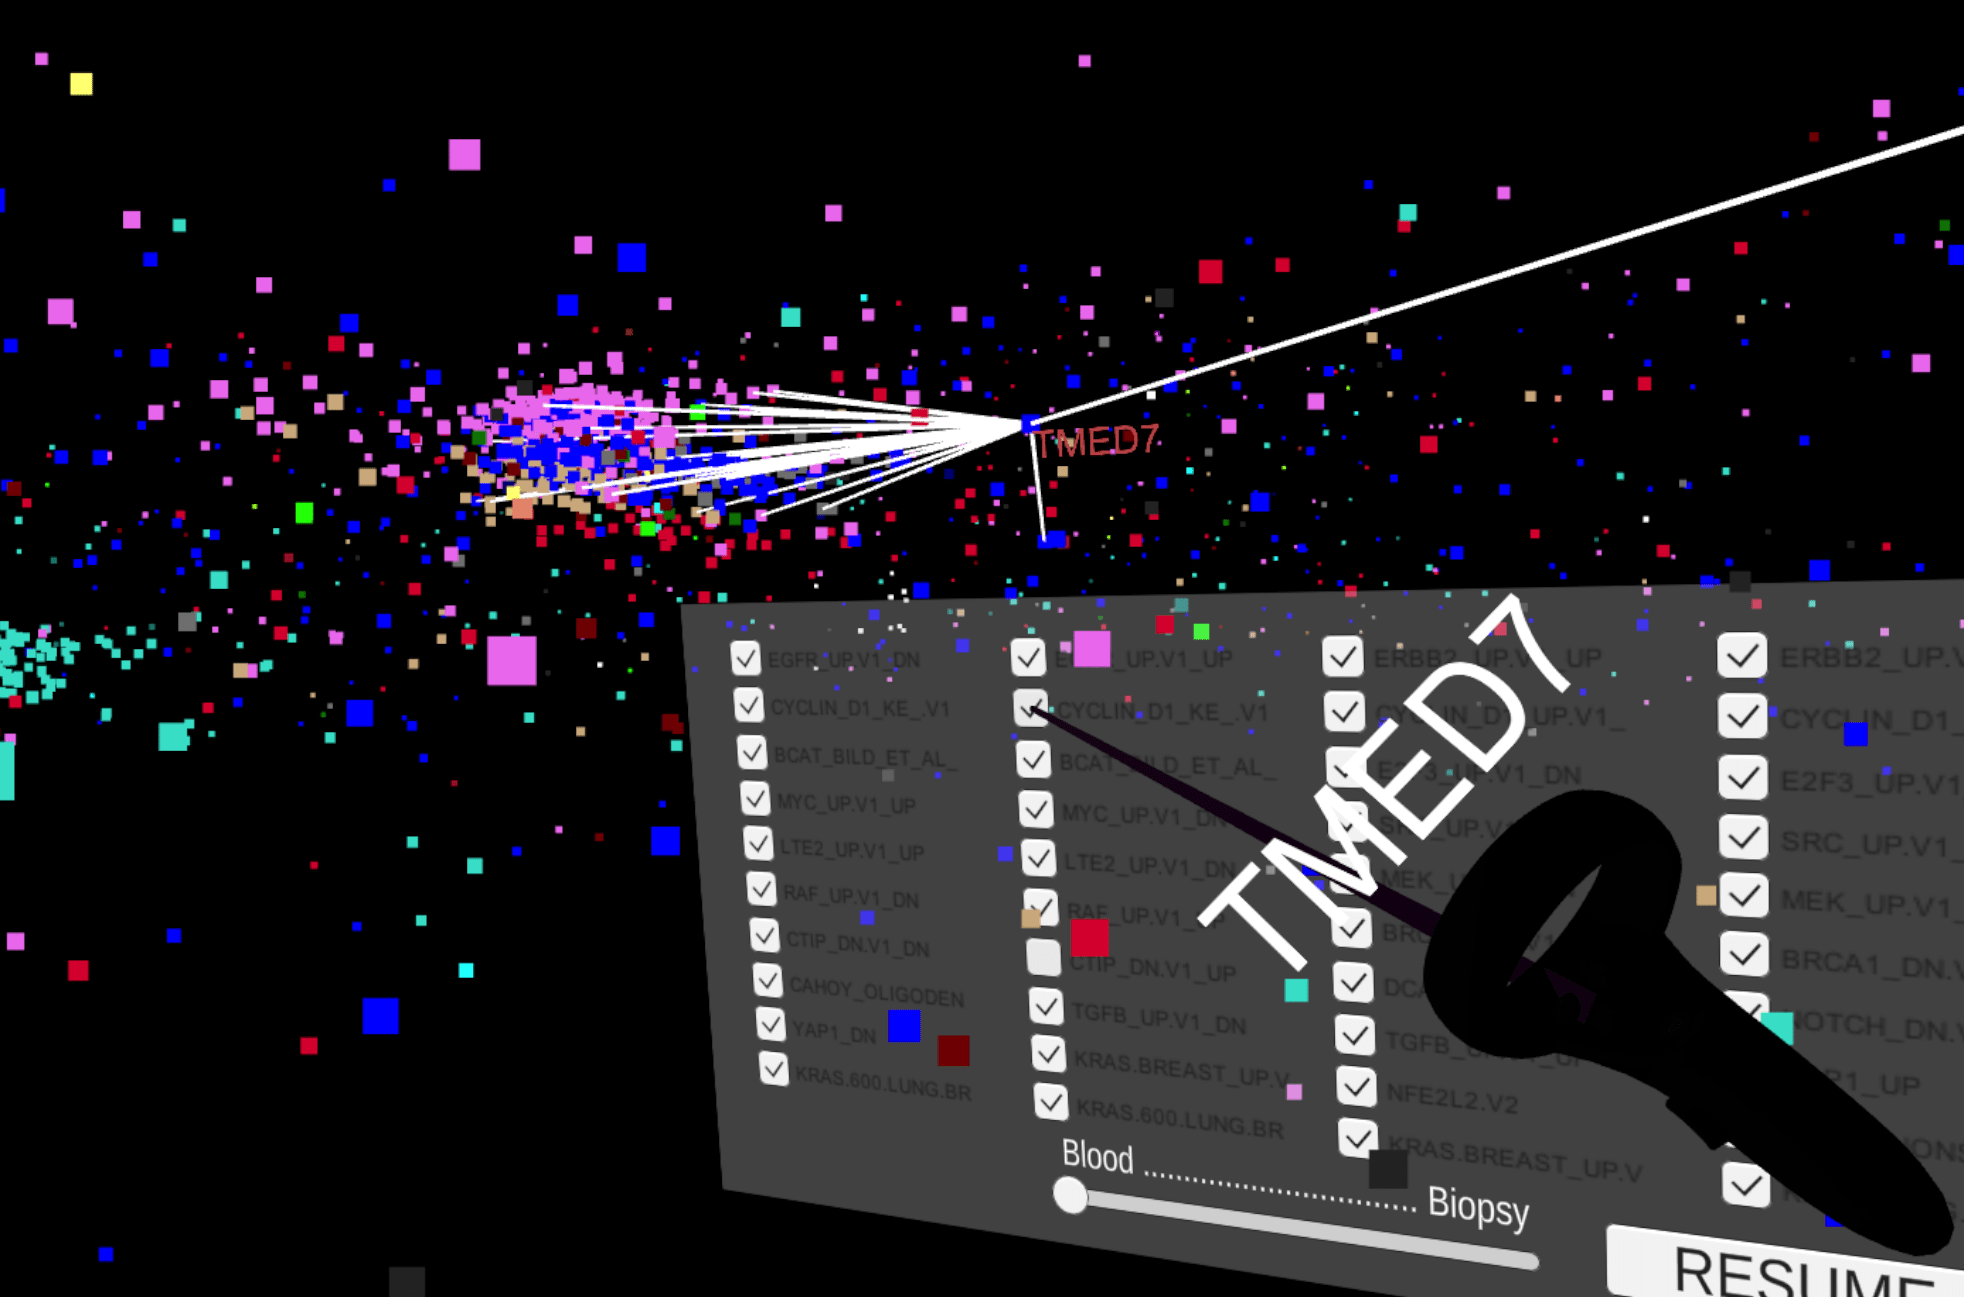
\includegraphics[width=\textwidth]{mixt_vr_introduction}
    \caption{A screenshot from GeneNet VR where a user is exploring the blood dataset from MIxT.}
    \label{fig:bignet_intro}
\end{figure}


\section{Outline}

We have structured the thesis in the following chapters: Chapter 2 describes how GeneNet VR was implemented, the architecture, design and the Virtual Reality techniques that were used. Chapter 3 focuses on explaining the visualization of MIxT in Virtual Reality and the datasets that we are using. In Chapter 4 we describe the experiments we carried out and our conclusions which we used in order to evaluate GeneNet VR. Chapter 5 describes some related projects found in scientific literature and we draw comparisons with GeneNet VR. In Chapter 6 we explain the conclusions from the project. In Chapter 7 we describe the future development ideas that we have for GeneNet VR.
